% ----------------------------------------------	
\pagestyle{plain}
\whitetext{\chapter{Introduction}}
\pagecolor{ccteal}
\fontfamily{phv}


\definecolor{insetbox_teal}{RGB}{230, 239, 239}
\colorbox{insetbox_teal}{
\begin{minipage}[b]{\textwidth}

\begin{table}[H]
\small

\input{\rootpath/TABLES/overview_table/\tds_overview_table}
\end{table}

\begin{centering}
\input{\rootpath/TABLES/typology_table/\tds_typology}
\end{centering}
\end{minipage}
}

%\vspace*{\stretch{.5}}
\pagebreak
\newpagecolor{white}
\pagestyle{fancy}
\fancyhf{}
\renewcommand{\chaptermark}[1]{\markboth{#1}{}}
\fancyfoot[LE,RO]{\thepage}

	\begin{minipage}[t][.39\textheight][t]{\textwidth}
	\textcolor{ccteal}{\section{Overview}}
	\input{\rootpath/TEXT/overview_text/\tds_overview}
	
	\end{minipage}


\pagebreak

\newgeometry{left=0in, right=0in, top=0in, bottom=0in}
\fakesection{Context Map}
\afterpage{%
    \clearpage% flush all other floats
    \ifodd\value{page}
    %\else% uncomment this else to get odd/even instead of even/odd
        \expandafter\afterpage% put it on the next page if this one is odd
    \fi
    {%
    \begin{figure}[H]
    	\raggedleft
        \includegraphics[height=11in]{\rootpath/MAPS/context_maps/\tds_context_1.png}%
    \end{figure}
    \clearpage
    \begin{figure}[H]
    	\raggedright
        \includegraphics[height=11in]{\rootpath/MAPS/context_maps/\tds_context_2.png}%
    \end{figure}
    \clearpage
    }%
}
\restoregeometry
\pagebreak
%-------------------------------------------
\pagestyle{plain}
\whitetext{\chapter{Waste Services and Assets}}
\pagecolor{ccorange}

\pagebreak
%\newgeometry{right=0in}
\newpagecolor{white}
\pagestyle{fancy}
\fancyhf{}
\renewcommand{\chaptermark}[1]{\markboth{#1}{}}
\fancyfoot[LE,RO]{\thepage}
\parbox[T][3in][c]{\textwidth}{
\textcolor{ccorange}{\section{Waste Distribution}}
%%%% TO-DO: AUTOMATE TEXT GENERATION %%%
\input{\rootpath/TEXT/waste_distribution_top/\tds_wd_top.tex}
}

\begin{table}[H]
\begin{threeparttable}
\small

\input{\rootpath/TABLES/waste_distribution_table/\tds_wd_table_1}

\end{threeparttable}
\end{table}
\pagebreak
%\newgeometry{left=0in, right=.5in, top=.5in, bottom=.5in}
\parbox[T][3in][c]{\textwidth}{
\input{\rootpath/TEXT/waste_distribution_bottom/\tds_wd_bottom.tex}}
\begin{table}[H]
\begin{threeparttable}
\small

\input{\rootpath/TABLES/waste_distribution_table/\tds_wd_table_2}

\begin{tablenotes}
\item [1] Assumes 5lbs of waste is produced daily in each unit.
\item [2] Includes miscellaneous garbage as well as uncaptured recyclables, organics, e-waste, and textiles.
\item [3] Primary method of trash collection, via chute. Assumes a 75\% capture rate.
\item [4] Secondary method of trash collection. Assumes a 25\% capture rate
\item [5] Capture rates of recyclables at NYCHA portfolio-wide: 30\% of MGP, 50\% of Cardboard, and 20\% of Paper. 
%\item[5] Organics, e-waste, and textiles have a capture rate of 0\%.
\end{tablenotes}
\end{threeparttable}
\end{table}


\pagebreak
\restoregeometry
%\KOMAoptions{paper=letter, paper=portrait}
%\recalctypearea
\textcolor{ccorange}{\section{Waste Services and Assets}}
%%% TO-DO: AUTOMATE TEXT GENERATION %%%
At sites where household waste is not picked up curbside, caretakers are responsible for transporting waste from internal compactor rooms and secondary collection sites to external compactors, either at the development in question or another development within the consolidation. As a rule, bulk is transported to a central location in each consolidation for pickup, while recyclables are collected curbside.
\begin{table}[H]
\small
%%% TO-DO: AUTOMATE WASTE SERVICES AND ASSETS TABLE %%%
%%%%%%%%%%%%%%%%%%%%%%%%%%%%%%%%%%%%%%%%%%%%%%%%%%%%%%%%%%%%%%%%%%%%%
\small
\input{\rootpath/TABLES/waste_services/\tds_waste_services_1.tex}
\bigskip
\input{\rootpath/TABLES/waste_services/\tds_waste_services_2.tex}
\end{table}
\pagebreak

\textcolor{ccorange}{WASTE ASSET MAP}
\begin{figure}[H]
\raggedright
\includegraphics[width=.95\textwidth]{\rootpath/MAPS/asset_maps/\tds_asset_map.png}
\end{figure}
\pagebreak

\textcolor{ccorange}{WASTE ASSETS}

\begin{table}[H]
\begin{threeparttable}
\small

\input{\rootpath/TABLES/waste_assets/\tds_waste_assets}

\begin{tablenotes}
\item [1] Recycling bin data may be incomplete; consult with development staff before using.
\end{tablenotes}
\end{threeparttable}
\end{table}

\textcolor{ccorange}{SUMNER CONSOLIDATION ASSETS}
\begin{table}[H]
\begin{tabular}{m{.33\columnwidth}m{.33\columnwidth}m{.33\columnwidth}}
{\color{ccorange} X Trucks} & {\color{ccorange} X Bobcats} & {\color{ccorange} X Other} \\

\includegraphics[width=.25\columnwidth]{\rootpath/IMAGES/truck.png}                            & 
\includegraphics[width=.25\columnwidth]{\rootpath/IMAGES/bobcat.png}                             & 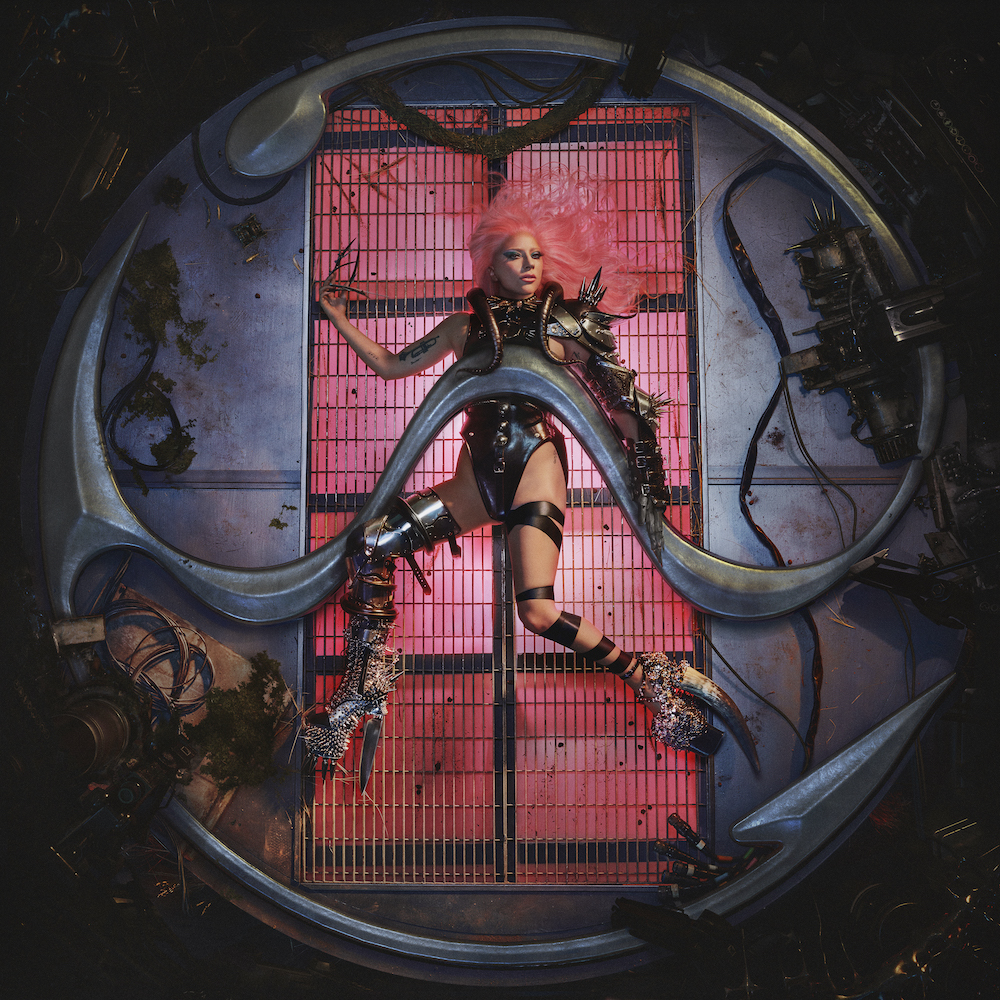
\includegraphics[width=.25\columnwidth]{\rootpath/IMAGES/chromatica.jpg}                          
\end{tabular}
\end{table}
\pagebreak
\textcolor{ccorange}{\section{Capital Improvements}}


\begin{table}[H]
%\resizebox{\textwidth}{\textheight}{
\small
\begin{tabular}{l}
\input{\rootpath/TABLES/capital_projects_table/\tds_capital_projects_1}\\
\input{\rootpath/TABLES/capital_projects_table/\tds_capital_projects_2}
\end{tabular}
%}
\end{table}
\pagebreak

\textcolor{ccorange}{PRIORITIES}

PLACEHOLDER TEXT AND TABLES AND SUCH TO FIGURE OUT PAGE COLOR SETTINGS -- WILL FILL IN LATER, ONCE PRELIMINARY ANALYSIS IS COMPLETE
\pagebreak
%-------------------------------------------
\pagestyle{plain}
\whitetext{\Chapter{Staffing}}
\pagecolor{ccfuschia}
\pagebreak
\newpagecolor{white}
\pagestyle{fancy}
\fancyhf{}
\renewcommand{\chaptermark}[1]{\markboth{#1}{}}
\fancyfoot[LE,RO]{\thepage}


\textcolor{ccfuschia}{STAFFING STRUCTURE}
\begin{figure}[H]
	\resizebox{\textwidth}{!}{
	\centering
	\begin{tikzpicture}[node distance=3cm]
	\node (vp) [processwide] {VP of Operations};
	\node (borodr) [processwide, below of=vp] {Borough Director};
	\node(ram) [processwide, below of=borodr] {Regional Asset Manager};
	\node (pm) [processwide, below of=ram] {Property Manager};
	\node (super) [process, below of=pm, xshift=-5cm] {Superintendent};
	\node (asuper) [process, below of=super] {Assistant Superintendent};
		\node (mtn) [process, below of=asuper, xshift=-3.5cm] {Maintenance Workers};
		\node (spc) [process, below of=asuper] {Supervisor of Caretakers};
			\node (crt) [process, below of=spc] {Caretakers\\(X and J)};
		\node (spg) [process, below of=asuper, xshift=3.5cm] {Supervisor of Grounds};
			\node (crtg) [process, below of = spg] {Caretakers (G)};			
		
	\node (apm)[process, below of=pm, xshift=5cm] {Assistant Property Manager};
		\node (sec) [process, below of=apm, xshift = -2.5cm] {Secretaries};
		\node (asst) [process, below of=apm, xshift = 2.5cm] {Housing Assistants};

	%\node (sub1) [subprocess, below of=pro1] {\nodepart{two} Subprogram};
	%\node (dec1) [decision, below of=sub1, yshift=-1cm] {Decision};
	%\node (com1) [comment, below of=dec1, xshift=-4cm, yshift=-1cm] {STEP 2};
	%\node (stop) [startstop, below of=dec1, yshift=-1cm] {Stop};

	%\draw [arrow] (dec1.west) -- ++(-1,0) node[anchor=south,pos=0.5] {No} |- (sub1.west);
	%\draw [arrow] (dec1) -- node[anchor=west] {Yes} (stop);

	\draw [arrow] (vp) -- (borodr);
	\draw [arrow] (borodr) -- (ram);
	\draw [arrow] (ram) -- (pm);
	\draw [arrow] (pm) -- (super);
	\draw [arrow] (super) -- (asuper);
		\draw [arrow] (asuper) -- (mtn);
		\draw [arrow] (asuper) -- (spc);
			\draw [arrow] (spc) -- (crt);
		\draw [arrow] (asuper) -- (spg);
			\draw [arrow] (spg) -- (crtg);
	
	\draw [arrow] (pm) -- (apm);
		\draw [arrow] (apm) -- (sec);
		\draw [arrow] (apm) -- (asst);
	\end{tikzpicture}
	}
\end{figure}

\pagebreak
\textcolor{ccfuschia}{ALLOCATED STAFF}

\begin{table}[H]
\begin{threeparttable}

\input{\rootpath/TABLES/staff_table/\tds_staff_table}

\begin{tablenotes}
\item [1] Includes staff in roles Caretaker J, Caretaker I, and Chief Caretaker
\end{tablenotes}
\end{threeparttable}
\end{table}

\pagebreak
%-------------------------------------------
\pagestyle{plain}
\whitetext{\Chapter{Analysis}}
\pagecolor{ccgreen}
\pagebreak
\newpagecolor{white}
\pagestyle{fancy}
\fancyhf{}
\renewcommand{\chaptermark}[1]{\markboth{#1}{}}
\fancyfoot[LE,RO]{\thepage}
\textcolor{ccgreen}{ANALYSIS OF FINDINGS}
\\
\input{\rootpath/TEXT/analysis_text/\tds_analysis}

\pagebreak
% ############################################
\pagestyle{plain}
\whitetext{\Chapter{Appendices}}
\pagecolor{lightBlue}
\pagebreak
\newpagecolor{white}
\pagestyle{fancy}
\fancyhf{}
\renewcommand{\chaptermark}[1]{\markboth{#1}{}}
\fancyfoot[LE,RO]{\thepage}
\textcolor{darkBlue}{Appendix I}

PLACEHOLDER

\pagebreak

% ############################################

% ############################################
\begin{comment}

\section{Lists}

Unordered Lists:
\begin{itemize}
\item This is an unordered list. 
\item Item 2.
\item It has three items.
\end{itemize}

Ordered List:
\begin{enumerate}
\item This is an ordered list.
\item Item 2.
\item It has three items.
\end{enumerate}

Ordered List (alphabetical):
\begin{enumerate}[label=\Alph*.]
\item This is an ordered list.
\item Item 2.
\item It has three items.
\end{enumerate}

% ----------------------------------------------
\cleardoublepage
\chapter{Figures}\label{ch:figures}

% ############################################
\section{Images}\label{sec:images}

\autoref{fig:image1} shows how to display images.

\begin{figure}[H]
	\centering
	\includegraphics[width=0.5\textwidth]{example-image-a.pdf}
	\caption{Image}

	\label{fig:image1}
\end{figure}

\begin{figure}[H]
	\centering
	\includegraphics[width=0.5\textwidth]{example-image-b.pdf}
	\caption{Image with Source}
	\captionsource{\cite{mus:16}}	
	\label{fig:image2}
\end{figure}

\begin{figure}[H]
	\centering
	\includegraphics[width=0.5\textwidth]{example-image-c.pdf}
	\caption{Image with Source and Link}
	\captionsource[https://example.org]{J. Doe}	
	\label{fig:image3}
\end{figure}

% ############################################

% ----------------------------------------------
\cleardoublepage
\chapter{Conclusion}\label{ch:conclusion}

\end{comment}

